\section{Datacrawler}
\label{Datacrawler}
The main goal of the datacrawler is to deliver the required datasets as specified in chapter \ref{datasets}. The input to the datacrawler is simply a domain, which is provided by the ground truth. Depending on the configuration the output of the datacrawler can vary from a single screenshot (\ref{DatasetVersion1}) to a complete graph of the given domain (\ref{DatasetVersion2}).

The following section (\ref{datacrawler_requirements}) will profoundly discuss the requirements in functionality for the datacrawler, which will serve as a basis for discussion for the decision between the frameworks \texttt{Puppeeter} and \texttt{Chromium Embedded Framework} (\ref{datacrawler_framework_language}). Afterwards we will give an overview of the architecture (\ref{datacrawler_architecture}) and highlight the idea of \textit{DataModules} in the crawler (\ref{datacrawler_datamodulesystem}). Following that, we will discuss profoundly all developed \textit{DataModules} with their role in the datacrawler (\ref{datacrawler_screenshot_datamodule}, \ref{datacrawler_mobilescreenshot_datamodule}, \ref{datacrawler_url_datamodule}). We will wrap up the internals of the datacrawler by taking a look into the workflow of the datacrawler (\ref{datacrawler_workflow}).

In the last section (\ref{datacrawler_scale}) we will discuss how we successfully designed a sophisticated system to scale-out the datacrawler reducing the total dataset creation time on Google Cloud Platform.  

\subsection{Requirements}
\label{datacrawler_requirements}
The requirements in functionality for the datacrawler arise from the dataset specifications (\ref{DatasetVersion1}, \ref{DatasetVersion2}). The next section will derive the requirements from the dataset specifications and discuss them profoundly.

\subsubsection{Browser Emulation}
\label{browser_emulation}
One of the major requirements for the datacrawler is to find a convenient way of emulating a web browser. According to the dataset specifications, for every given website a screenshot $\tensorsym{I}$ has to be taken. In addition to that, every screenshot must represent the website as the user would see in a common browser. The latter and other attributes such as the loading time $l$ of a website like in a common browser make the emulation of a browser an inevitable requirement. 

\subsubsection{Information Accessibility}
\label{information_accessibility}
Accessing \textit{low-level} information such as the \textit{HTTP-Request} to change the \textit{user-agent} to generate a mobile screenshot $\tensorsym{M}$ (\ref{datacrawler_mobilescreenshot_datamodule}) or the \textit{Document Object Model (DOM)} (\ref{datacrawler_url_datamodule}) to generate edges $a$ in the graph according to dataset version 2 specification (\ref{DatasetVersion2}) is inevitable. The datacrawler has to be able to manipulate internal data structures and even able to inject own \textit{JavaScript-code} (\ref{datacrawler_screenshot_datamodule}) on the website.

\subsubsection{Modularity}
\label{modularity}
The datacrawler has to be as modular for allowing us to extend the datacrawler easily and decide which attribute should be calculated. This requirement in flexibility is raised from the fact that our dataset specifications might change over the time or new ones might be added.

This flexibility led to a sophisticated architecture such as the \text{DataModule-System} (\ref{datacrawler_datamodulesystem}), which makes it possible to pass the dataset specification directly into the datacrawler.

\subsubsection{Scalability}
\label{scalability}
Both dataset versions require the analysis of at least 100,000 websites. Therefore, datacrawler has to be horizontally scalable to allow the analysis of multiple domains at once, and efficient in terms analysis time and start-up time. An inefficient and not scalable datacrawler would lead to multiple days of required analysis time and reflect also in high infrastructure costs.

\subsection{Framework}
\label{datacrawler_framework_language}
The previous section has shown some of the intricate requirements for the datacrawler. To answer those requirements in the given time frame, we investigated in frameworks, which would do most of the heavy-lifting for us such as networking, I/O or rendering of the website.

In our research we focused on the evaluation of frameworks, which base on the most common browser \texttt{Google Chrome} \cite{CommonBrowsers}. This section will introduce two frameworks \texttt{Puppeteer} and \texttt{Chromium Embedded Framework} (\texttt{CEF}), compare both and discuss our decision for \texttt{CEF}. Both frameworks are providing an API to instrument the well-known browser \texttt{Chrome}.

\subsubsection{Puppeteer}
\texttt{Puppeteer} is a open-source library for the JavaScript runtime \texttt{Node.js}, which provides a high-level API to control instances of the browsers \texttt{Chrome} or \texttt{Chromium}. One of the main goals of \texttt{Puppeteer} is to grow adoption in automated browser testing \cite{PuppeteerFAQ}.  For this purpose, it wraps the \texttt{Chrome DevTools Protocol} in JavaScript, which allows web developers to instrument, inspect and debug instances of \texttt{Chrome}. Technically, the protocol is HTTP-based and exposed as a RESTful API at the port for debugging by \texttt{Chrome}.

The protocol offers a varies number of functionalities, which are grouped into domains \cite{DevToolsProtocol}. Some of the interesting domains for our use-case are:
\begin{description}
	\item[Page]: API to load and take a screenshot of the given website.
	\item[DOM]: API to read and manipulate the DOM of the given website.
	\item[Network]: API to intercept network requests, track downloaded data and network issues.
	\item[Emulation]: API to emulate different geolocation, network bandwith and mobile devices.
\end{description}

During start up \texttt{Puppeteer} starts an instance of \texttt{Chrome}, attaches to the instances using the port for debugging and afterwards custom code of the user will be executed against the instance. The instance will be started in \texttt{headless}-mode meaning that no UI will be visible.

\texttt{Puppeteer} fulfills all requirements (\ref{datacrawler_requirements}) raised from the dataset specifications:
The requirement of \textbf{Browser Emulation} (\ref{browser_emulation}), since it is using an instance of \texttt{Chrome} to render websites. The requirement of \textbf{Information Accessibility} (\ref{information_accessibility}), due to functionalities in the domains DOM and Network. Furthermore \textbf{Modularity} (\ref{modularity}) is given per se by using JavaScript as the programming language, which makes the use of polymorphism possible as used in DataModule-System (\ref{datacrawler_datamodulesystem}). The usage of \texttt{Chrome} ensures efficiency in terms of loading, rendering websites and retrieval of website information. Moreover, the combination of \texttt{Chrome} and \texttt{Puppeteer} can be scaled-out easily fulfilling the last requirement \textbf{Scalability} (\ref{scalability}) by using our system described in \ref{datacrawler_scale}.

\subsubsection{Chromium Embedded Framework}
\texttt{Chromium Embedded Framework (CEF)} is an open-source framework for embedding the \texttt{Chromium} browser into other applications. The main goal of \texttt{CEF} is to enable developers in adding web browsing functionality such as using HTML, CSS and JavaScript to create application UI. Well-known applications such as \texttt{Adobe Acrobat}, \texttt{Spotify Desktop} and \texttt{MATLAB} are using \texttt{CEF}.

\texttt{CEF} was designed ground-up with performance and ease-use in mind. The framework exposes \texttt{C++} interfaces with default implementation for all features requiring little or no integration work. Furthermore, the community added wrappers for the base implementation to support a wide-range of operating systems and programming languages.

\texttt{CEF} has in total three versions, whereas \texttt{CEF 2} was abandoned due to the appearance of the \texttt{Chromium Content API} which will be discussed later. \texttt{CEF 1} is a single process implementation and based on the old \texttt{Chromium WebKit API}, due to deprecation of the \texttt{Chromium WebKit API} it is no longer supported and developed. \texttt{CEF 3} is a multi process implementation and based on the current \texttt{Chromium Content API}.

As the \texttt{Chromium} code base has grown, it was inevitable to avoid opaque dependencies and features in the wrong places. Therefore the \textit{content module} was introduced, which contains the core functionality of \texttt{Chromium}. The \texttt{Chromium Content API} wraps the \texttt{content module} and offers isolation for developers from the core functionalities \cite{ChromiumContentAPI}.
\texttt{CEF 3} insulates the user from the underlying complexity of \texttt{Chromium} by using the \texttt{Chromium Content API} and offering production-quality stable APIs \cite{CEFGeneralUsage}. The offered and consumed APIs as well as the multi-process architecture will be profoundly discussed in \textbf{Datacrawler Architecture} (\ref{datacrawler_architecture}).

Through the use of \texttt{Chromium Content API}, \texttt{CEF 3} provides a close integration between the browser and the host application including support for custom JavaScript objects and JavaScript extensions. Moreover, the host application is able to control resource loading, intercept the network, navigation and many more, while taking advantage of the same performance and technologies available in the \texttt{Google Chrome Web browser} \cite{CEFGeneralUsage}.

\texttt{CEF 3} clearly fulfills the requirement of \textbf{Browser Emulation} (\ref{browser_emulation}) and \textbf{Information Accessibility} (\ref{information_accessibility}). Moreover, \textbf{Modularity} (\ref{modularity}) and \textbf{Scalability} (\ref{scalability}) is also given by using \texttt{C++} and the core functionalities of \texttt{Chromium}.

\subsubsection{Framework Decision}
Both \texttt{Puppeteer} and \texttt{CEF} fulfill the requirements raised by the dataset specifications. At first glance it seemed a free choice, but after close investigation we found additional points speaking for \texttt{CEF}. In the end we decided to use \texttt{CEF 3} for the datacrawler, due to following additional points:
\begin{itemize}
\item Our team has an outstanding expertise in \texttt{C++}, which is the programming language used in both \texttt{CEF 3} and \texttt{Chromium}.
\item While as \texttt{Puppeteer} is limited to the \texttt{Chrome DevTools Protocol}, \texttt{CEF 3} provides low-level access to the core of \texttt{Chromium}. This ultimately gives us more freedom of control.
\item \texttt{CEF 3} is integrated into \texttt{Chromium} leading to a faster start-up and execution time Whereas \texttt{Puppeteer} has to start up an instance of \texttt{Chrome} and communicate via a RESTful HTTP API, which represents an addition overhead.
\end{itemize}
\subsection{Datacrawler Architecture}
\label{datacrawler_architecture}
One of the major points in the design and implementation of the Datacrawler was to meet the \textbf{Modularity} requirement (\ref{modularity}). This led to the development of the sophisticated \textit{DataModule}-System and introduced the concept of \textit{Datamodules}. The Datamodule-System represents the architecture of the Datacrawler. 

Before diving into our implementation details by introducing the \textit{DataModule}-System, we will discuss how applications using \texttt{CEF 3} are build and work in general (\ref{datacrawler_cef_architecture}). Following that, we will introduce the \textit{DataModule}-System (\ref{datacrawler_datamodulesystem}) in great detail giving the required information to understand how \textit{Datamodules} work. Afterwards we will discuss how we take a screenshot of a website and tackle the challenge of detecting when a website has finished loading in the \textit{Screenshot}-Datamodule (\ref{datacrawler_screenshot_datamodule}). Beyond that we will discuss how we take screenshots by emulating a mobile device (\ref{datacrawler_mobilescreenshot_datamodule}) and collect URLs by traversing the DOM (\ref{datacrawler_url_datamodule}). In the end we will show how we generate and output the graph (\ref{datacrawler_graph}) and wrap up by taking a look into the end-to-end workflow of the Datacrawler (\ref{datacrawler_workflow}). 

\subsubsection{CEF 3 Application Structure}
\label{datacrawler_cef_architecture}
\texttt{CEF 3} is based on multiple processes. It can mainly be divided into the \textit{browser}-process and \textit{render}-process.

\begin{itemize}
\item The browser-process represents the host process of the application, which handles window creation, painting and network access. Furthermore, most of the application logic will run in the browser-process. 
\item Multiple render-processes are responsible for rendering websites, executing JavaScript and running some application logic. Following the process model of \texttt{Chrome}, \texttt{CEF 3} spawns for every unique origin a render-process ensuring resource isolation, parallelism and better failure management.
\end{itemize}

The separate spawned processes communicate using \textit{Inter-Process Communication} (IPC). Application logic implemented in browser- and render-process can communicate by sending asynchronous messages as \textbf{URL-Datamodule} (\ref{datacrawler_url_datamodule})  will show. Other processes are spawned when needed such as the \textit{plugin}-process for handling of plugins like \textit{Flash}.

In general \texttt{CEF 3} application consists of the class \texttt{CefApp} and \texttt{CefClient}. \texttt{CefApp} is responsible for process-specific callbacks such as returning handler for a custom render-process implementation (\ref{datacrawler_url_datamodule}). Whereas \texttt{CefClient} is responsible for handling browser-instance-specific callbacks such as returning handler for a customer website render implementation (\ref{datacrawler_screenshot_datamodule}). It contains most of the application logic and is being used to create browser instances. As mentioned before, it can be used to control the browser-instance with custom implementation.

The following will briefly describe the start-up of an application using \texttt{CEF 3}:
\begin{enumerate}
	\item The \texttt{CefExecuteProcess}-method is used with custom implementation of \texttt{CefApp} to start separate processes. The application executable will be started multiple times representing new processes.
	\item \texttt{CreateBrowser} is used with custom implementation of \texttt{CefClient} to create a browser-instance. The browser instance is created in the browser-process, which means that there is only one browser at a time. Futhermore, an initial URL is passed to the browser-instance.
	\item In the implementation of \texttt{CefClient} \texttt{CefMessageLoop}-method is executed, which starts the event loop of the browser-instance. This means that browser-instance will start loading the given URL, handling network, rendering and many more. \texttt{CEF} takes care of spawning and using of existing render-processes.
	\item Once \texttt{CefQuitMessageLoop}-method is called, the message loop will be quit.
\end{enumerate}

\subsubsection{DataModule-System}
\label{datacrawler_datamodulesystem}
The naming of the DataModule-System derives from the use of Datamodules and represents the core of the Datacrawler. The system consists of several components, which enable developers to implement and test Datamodules independently increasing flexibility and reducing potential failures. In a plugin-and-play-manner developers can easily develop and add Datamodules to the Datacrawler.

The main idea of a Datamodule is to represents a single attribute in the dataset, which is calculated and added independently from other attributes to the dataset. In addition, each Datamodule can be individually configured and turned on or off by the user.

In order for a Datamodule to be executable, it has to implement following interfaces:

\begin{itemize}
	\item[DataModuleBaseConfiguration] description
	\item[DataModulebase] description
	\item[DataBase] description
\end{itemize}

\begin{figure}[h]
	\centering
	 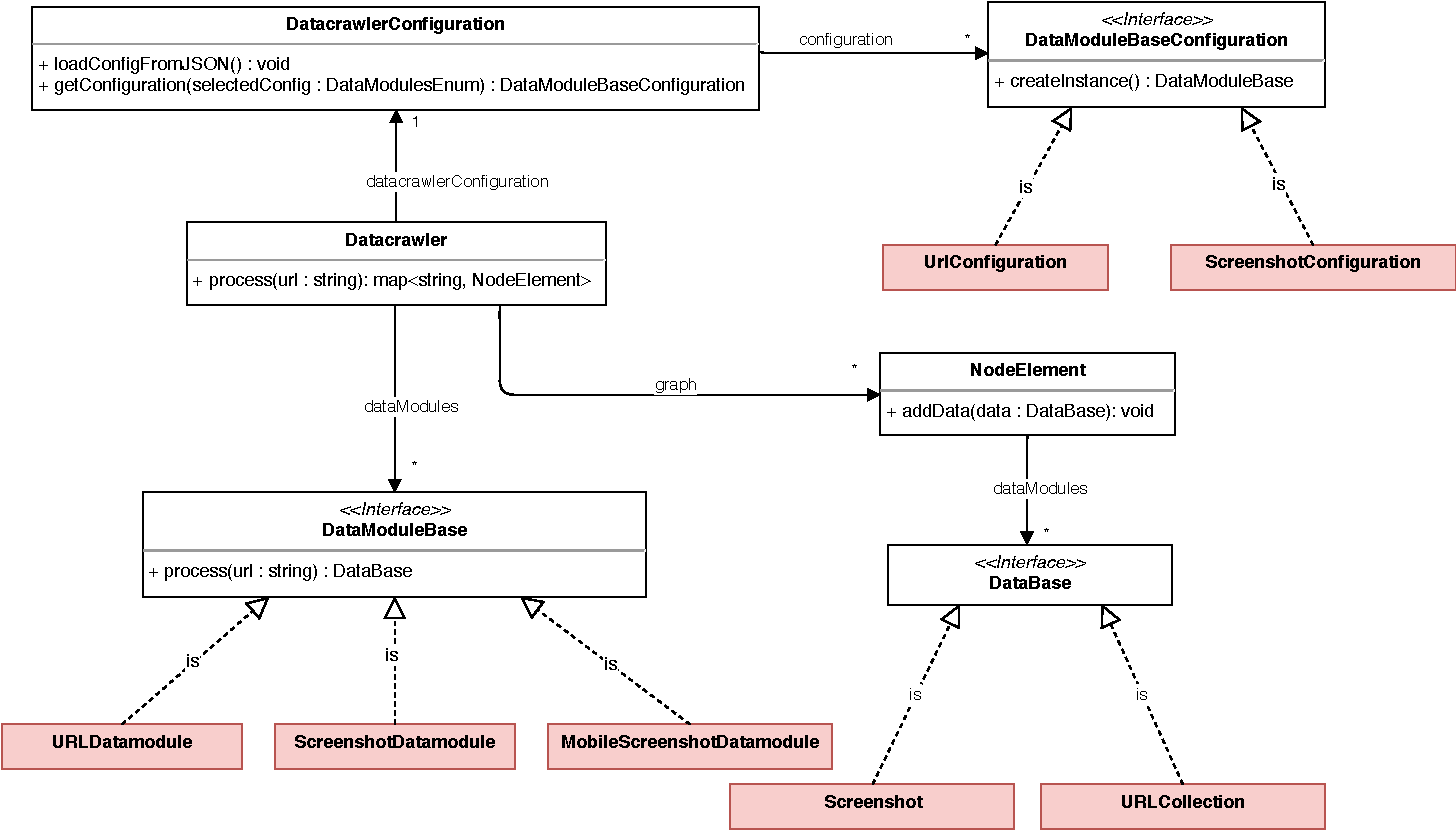
\includegraphics[scale=0.65]{resources/datacrawler_uml_diagram}
	 \caption{The figure shows the simplified UML-diagram of the datacrawler with the most prominent classes and methods. Classes in the white boxes represent essential components of the DataModule-System such as the classes \textit{Datacrawler}, \textit{DatacrawlerConfiguration}, \textit{NodeElement} and the interfaces \textit{DataModuleBaseConfiguration}, \textit{DataModulBase} and \textit{DataBase}. Classes in the red boxes represent implementation of DataModules such as the \textit{URLDatamodule} (\ref{datacrawler_url_datamodule}), \textit{ScreenshotDatamodule} (\ref{datacrawler_screenshot_datamodule}) and \textit{MobileScreenshotDatamodule} (\ref{datacrawler_mobilescreenshot_datamodule}).}
	\label{fig:datacrawler_uml_diagram}
\end{figure}

\subsubsection{Screenshot-Datamodule}
\label{datacrawler_screenshot_datamodule}

\subsubsection{MobileScreenshot-Datamodule}
\label{datacrawler_mobilescreenshot_datamodule}

\subsubsection{URL-Datamodule}
\label{datacrawler_url_datamodule}

\subsubsection{Generating the Graph}
\label{datacrawler_graph}
\subsubsection{Datacrawler Workflow}
\label{datacrawler_workflow}

In general Datacrawler can be divided mainly into three functional parts:

\begin{enumerate}
	\item[Initializiation] : The Datacrawler reads the Datamodule configuration from a local file and initializes the Datamodules accordingly.
	\item[Crawling] : The Datacrawler crawls the passed domain according to the activated Datamodules and calculates attributes for the dataset.
	\item[Output] : The Datacrawler generates and saves the graph to the disk.
\end{enumerate}


\subsection{Scaling the Datacrawler}
\label{datacrawler_scale}

\subsubsection{Requirements}
\label{datacrawler_scale_requirements}

\subsubsection{The Scale Architecture}
\label{datacrawler_scale_architecture}


